\documentclass{standalone}
\usepackage{tikz}
\usetikzlibrary{patterns, positioning}
\usepackage[sfdefault]{ClearSans} %% option 'sfdefault' activates Clear Sans as the default text font
\usepackage[T1]{fontenc}

\begin{document}
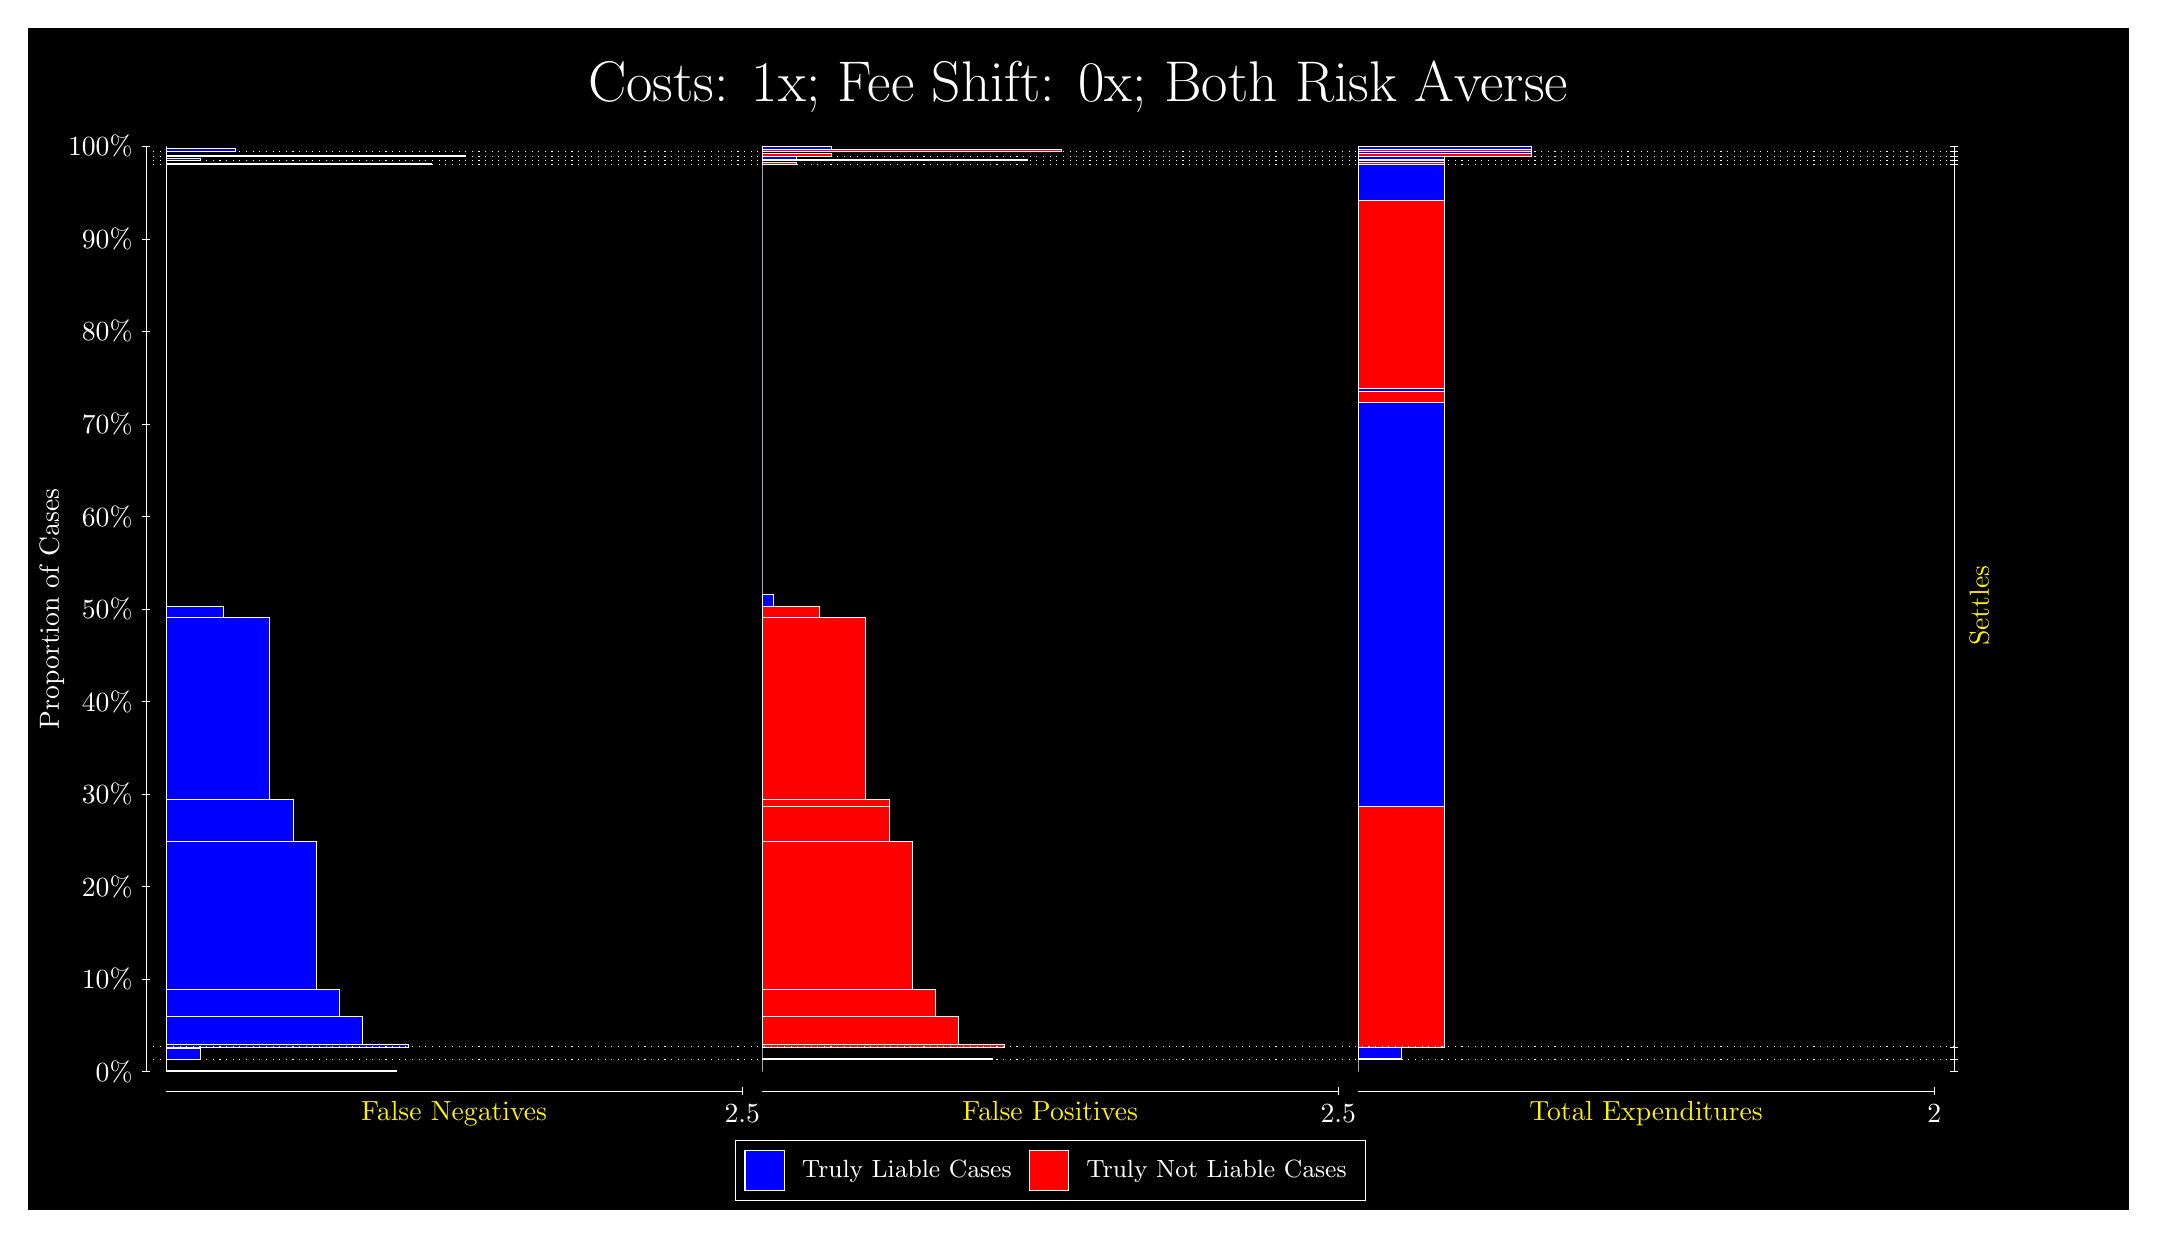
\begin{tikzpicture}
\draw[fill=black] (0,0) rectangle (26.667,15);
\draw[text=white] (0,13.5) rectangle (26.667,15) node[midway] {\huge Costs: 1x; Fee Shift: 0x; Both Risk Averse};
\draw[white, very thin] (1.5,1.75) -- (1.5,13.5);
\node[rotate=90, text=white, anchor=center] at (0.3, 7.625) {Proportion of Cases};
\draw[white, very thin] (1.45,1.75) -- (1.55,1.75);
\node[text=white, anchor=east] at (1.45, 1.75) {0\%};
\draw[white, very thin] (1.45,2.925) -- (1.55,2.925);
\node[text=white, anchor=east] at (1.45, 2.925) {10\%};
\draw[white, very thin] (1.45,4.1) -- (1.55,4.1);
\node[text=white, anchor=east] at (1.45, 4.1) {20\%};
\draw[white, very thin] (1.45,5.275) -- (1.55,5.275);
\node[text=white, anchor=east] at (1.45, 5.275) {30\%};
\draw[white, very thin] (1.45,6.45) -- (1.55,6.45);
\node[text=white, anchor=east] at (1.45, 6.45) {40\%};
\draw[white, very thin] (1.45,7.625) -- (1.55,7.625);
\node[text=white, anchor=east] at (1.45, 7.625) {50\%};
\draw[white, very thin] (1.45,8.8) -- (1.55,8.8);
\node[text=white, anchor=east] at (1.45, 8.8) {60\%};
\draw[white, very thin] (1.45,9.975) -- (1.55,9.975);
\node[text=white, anchor=east] at (1.45, 9.975) {70\%};
\draw[white, very thin] (1.45,11.15) -- (1.55,11.15);
\node[text=white, anchor=east] at (1.45, 11.15) {80\%};
\draw[white, very thin] (1.45,12.325) -- (1.55,12.325);
\node[text=white, anchor=east] at (1.45, 12.325) {90\%};
\draw[white, very thin] (1.45,13.5) -- (1.55,13.5);
\node[text=white, anchor=east] at (1.45, 13.5) {100\%};

\draw[white, very thin] (24.457,1.75) -- (24.457,13.5);
\draw[white, very thin] (24.407,1.75) -- (24.507,1.75);
\node[anchor=west] at (24.407, 1.75) {};
\draw[white, very thin] (24.407,1.9062) -- (24.507,1.9062);
\node[anchor=west] at (24.407, 1.9062) {};
\draw[white, very thin] (24.407,2.0623) -- (24.507,2.0623);
\node[anchor=west] at (24.407, 2.0623) {};
\draw[white, very thin] (24.407,13.267) -- (24.507,13.267);
\node[anchor=west] at (24.407, 13.267) {};
\draw[white, very thin] (24.407,13.317) -- (24.507,13.317);
\node[anchor=west] at (24.407, 13.317) {};
\draw[white, very thin] (24.407,13.368) -- (24.507,13.368);
\node[anchor=west] at (24.407, 13.368) {};
\draw[white, very thin] (24.407,13.434) -- (24.507,13.434);
\node[anchor=west] at (24.407, 13.434) {};
\draw[white, very thin] (24.407,13.5) -- (24.507,13.5);
\node[anchor=west] at (24.407, 13.5) {};

\draw[white, very thin, fill=blue] (1.75,1.75) rectangle (4.6775,1.7664);
\draw[white, very thin, fill=red] (1.75,1.7664) rectangle (1.75,1.9062);
\draw[white, very thin, fill=blue] (1.75,1.9062) rectangle (2.1891,2.0459);
\draw[white, very thin, fill=red] (1.75,2.0459) rectangle (1.75,2.0623);
\draw[white, very thin, fill=blue] (1.75,2.0623) rectangle (4.8239,2.0943);
\draw[white, very thin, fill=blue] (1.75,2.0943) rectangle (4.2384,2.4467);
\draw[white, very thin, fill=blue] (1.75,2.4467) rectangle (3.9457,2.7988);
\draw[white, very thin, fill=blue] (1.75,2.7988) rectangle (3.6529,4.6705);
\draw[white, very thin, fill=blue] (1.75,4.6705) rectangle (3.3602,5.2015);
\draw[white, very thin, fill=blue] (1.75,5.2015) rectangle (3.0674,7.519);
\draw[white, very thin, fill=blue] (1.75,7.519) rectangle (2.4819,7.6646);
\draw[white, very thin, fill=red] (1.75,7.6646) rectangle (1.75,13.267);
\draw[white, very thin, fill=blue] (1.75,13.267) rectangle (5.1167,13.288);
\draw[white, very thin, fill=red] (1.75,13.288) rectangle (1.75,13.317);
\draw[white, very thin, fill=blue] (1.75,13.317) rectangle (2.1891,13.347);
\draw[white, very thin, fill=red] (1.75,13.347) rectangle (1.75,13.368);
\draw[white, very thin, fill=blue] (1.75,13.368) rectangle (5.5558,13.391);
\draw[white, very thin, fill=red] (1.75,13.391) rectangle (1.75,13.434);
\draw[white, very thin, fill=blue] (1.75,13.434) rectangle (2.6283,13.477);
\draw[white, very thin, fill=red] (1.75,13.477) rectangle (1.75,13.5);
\draw[white, very thin, fill=red] (9.3189,1.75) rectangle (9.3189,1.8897);
\draw[white, very thin, fill=blue] (9.3189,1.8897) rectangle (9.3189,1.9062);
\draw[white, very thin, fill=red] (9.3189,1.9062) rectangle (12.246,1.9226);
\draw[white, very thin, fill=blue] (9.3189,1.9226) rectangle (9.3189,2.0623);
\draw[white, very thin, fill=red] (9.3189,2.0623) rectangle (12.393,2.0943);
\draw[white, very thin, fill=red] (9.3189,2.0943) rectangle (11.807,2.4467);
\draw[white, very thin, fill=red] (9.3189,2.4467) rectangle (11.515,2.7988);
\draw[white, very thin, fill=red] (9.3189,2.7988) rectangle (11.222,4.6705);
\draw[white, very thin, fill=red] (9.3189,4.6705) rectangle (10.929,5.1248);
\draw[white, very thin, fill=red] (9.3189,5.1248) rectangle (10.929,5.2015);
\draw[white, very thin, fill=red] (9.3189,5.2015) rectangle (10.636,7.5191);
\draw[white, very thin, fill=red] (9.3189,7.5191) rectangle (10.051,7.6647);
\draw[white, very thin, fill=blue] (9.3189,7.6647) rectangle (9.4652,7.8103);
\draw[white, very thin, fill=blue] (9.3189,7.8103) rectangle (9.3189,13.267);
\draw[white, very thin, fill=red] (9.3189,13.267) rectangle (9.758,13.297);
\draw[white, very thin, fill=blue] (9.3189,13.297) rectangle (9.3189,13.317);
\draw[white, very thin, fill=red] (9.3189,13.317) rectangle (12.686,13.338);
\draw[white, very thin, fill=blue] (9.3189,13.338) rectangle (9.758,13.368);
\draw[white, very thin, fill=red] (9.3189,13.368) rectangle (10.197,13.411);
\draw[white, very thin, fill=blue] (9.3189,13.411) rectangle (9.3189,13.434);
\draw[white, very thin, fill=red] (9.3189,13.434) rectangle (13.125,13.457);
\draw[white, very thin, fill=blue] (9.3189,13.457) rectangle (10.197,13.5);
\draw[white, very thin, fill=red] (16.888,1.75) rectangle (16.888,1.8897);
\draw[white, very thin, fill=blue] (16.888,1.8897) rectangle (16.888,1.9062);
\draw[white, very thin, fill=red] (16.888,1.9062) rectangle (17.437,1.9226);
\draw[white, very thin, fill=blue] (16.888,1.9226) rectangle (17.437,2.0623);
\draw[white, very thin, fill=red] (16.888,2.0623) rectangle (17.986,5.1248);
\draw[white, very thin, fill=blue] (16.888,5.1248) rectangle (17.986,10.248);
\draw[white, very thin, fill=red] (16.888,10.248) rectangle (17.986,10.394);
\draw[white, very thin, fill=blue] (16.888,10.394) rectangle (17.986,10.426);
\draw[white, very thin, fill=red] (16.888,10.426) rectangle (17.986,12.82);
\draw[white, very thin, fill=blue] (16.888,12.82) rectangle (17.986,13.267);
\draw[white, very thin, fill=red] (16.888,13.267) rectangle (17.986,13.297);
\draw[white, very thin, fill=blue] (16.888,13.297) rectangle (17.986,13.317);
\draw[white, very thin, fill=red] (16.888,13.317) rectangle (17.986,13.338);
\draw[white, very thin, fill=blue] (16.888,13.338) rectangle (17.986,13.368);
\draw[white, very thin, fill=red] (16.888,13.368) rectangle (19.083,13.411);
\draw[white, very thin, fill=blue] (16.888,13.411) rectangle (19.083,13.434);
\draw[white, very thin, fill=red] (16.888,13.434) rectangle (19.083,13.457);
\draw[white, very thin, fill=blue] (16.888,13.457) rectangle (19.083,13.5);
\draw[white, dotted] (1.5,1.9062) -- (24.457,1.9062);
\draw[white, dotted] (1.5,2.0623) -- (24.457,2.0623);
\draw[white, dotted] (1.5,13.267) -- (24.457,13.267);
\draw[white, dotted] (1.5,13.317) -- (24.457,13.317);
\draw[white, dotted] (1.5,13.368) -- (24.457,13.368);
\draw[white, dotted] (1.5,13.434) -- (24.457,13.434);
\draw[white, very thin] (1.75,1.5) -- (9.0689,1.5);
\node[text=yellow, anchor=north] at (5.4094, 1.5) {False Negatives};
\draw[white, very thin] (9.0689,1.45) -- (9.0689,1.55);
\node[text=white, anchor=north] at (9.0689, 1.45) {2.5};

\draw[white, very thin] (9.3189,1.5) -- (16.638,1.5);
\node[text=yellow, anchor=north] at (12.978, 1.5) {False Positives};
\draw[white, very thin] (16.638,1.45) -- (16.638,1.55);
\node[text=white, anchor=north] at (16.638, 1.45) {2.5};

\draw[white, very thin] (16.888,1.5) -- (24.207,1.5);
\node[text=yellow, anchor=north] at (20.547, 1.5) {Total Expenditures};
\draw[white, very thin] (24.207,1.45) -- (24.207,1.55);
\node[text=white, anchor=north] at (24.207, 1.45) {2};



\node[text=yellow, centered, rotate=90] at (24.777, 7.6646) {Settles};





\draw (12.978300999999998,1.5) node[draw=none] (baseCoordinate) {};
\begin{scope}[align=center]
        \matrix[scale=0.5, draw=white, below=0.5cm of baseCoordinate, nodes={draw}, column sep=0.1cm]{
            \node[rectangle, draw, minimum width=0.5cm, minimum height=0.5cm, fill=blue] {}; &
            \node[draw=none, font=\small, text=white] (B) {Truly Liable Cases}; &
            \node[rectangle, draw, minimum width=0.5cm, minimum height=0.5cm, fill=red] {}; &
            \node[draw=none, font=\small, text=white] (B) {Truly Not Liable Cases}; \\
            };
\end{scope}

\end{tikzpicture}
\end{document}